%!TEX root = ../main.tex
\chapter{Introduction} \label{chp:intro}

\pagenumbering{arabic}
\setcounter{page}{1}

\begin{center}
\emph{``In theory there is no difference between theory and practice. In practice there is.''}
\end{center}
\hfill Yogi Berra~~~~~~~~

\section{A seemingly simple problem}

I remember the moment when I was first confronted with the problem of sums of random variables. I was tutoring introductory probability, and one of my students (whose full-time job was in insurance) asked about how to find the distribution of a sum of random variables. My response was that there were simple cases when the distribution of the sum was known (sums of exponentials or gammas were gamma distributed, sums of normals were normal); indeed, these kind of calculations featured prominently in the course's assignments. But, the student asked, what about all the other situations which didn't fit into these niches?

As it turns out, there are many solutions to this problem, yet none of the answers are as simple as the original question.
To be more specific about the problem, let us consider the standard procedure for statistical inference:
\begin{enumerate}
\item Collect data on the system of interest
\item Fit a statistical model to the data
\item Use the model to infer interesting quantities
\item (Optional) Perform sensitivity analysis on the inference
\end{enumerate}
Steps 1 and 2 are the application of statistical techniques, and fall outside the scope of this thesis. Step 3 involves calculating probabilities of events occurring (e.g.\ bankruptcy, catastrophic climate events, physical infrastructure failure, Internet infrastructure failure), and expectations of random variables (e.g.\ expected profit, expected throughput for a communications hub, expected intensity of earthquakes or cyclones).

To summarise, practitioners are interested in evaluating $\Prob(S < \gamma)$, or $\Exp[g(S)]$ for some function $g$, where $S = X_1 + \dots + X_d$ is the sum of $d$ summands. When $S$ is a \emph{compound sum}, that is, a sum of random variables where the number of summands is also random, then the same quantities need to be estimated but with different techniques. The calculation of $\Prob(S < \gamma)$ when $\gamma$ is either very large or very small is treated as a special case, called a \emph{rare-event problem}, since it poses unique challenges; rare-event problems are relevant for estimating the probability of Black Swan events (that is, situations which are so rare that we have no historical record of them occurring).

The goal of this thesis is to outline how one would answer real-world questions relating to sums of continuous random variables in an accurate and efficient way. This thesis will use numerical analysis, Monte Carlo methods, asymptotic analysis, and limit theorems.

The research was not undertaken with the goal of being solely dedicated to computational methods, it is simply the case that there tends to be (to a greater or lesser extent) a computational element to each solution. One can learn a great deal about how sums behave by performing asymptotic analysis of the relevant probabilities, expectations, and integral transforms; an exemplary example of this is the \emph{principle of the single big jump}, to be discussed in Section~\ref{sec:asymptotics}.
And since evaluating other types of distributions (like the maximum of a random vector) present similar challenges to sums, the research was not undertaken considering only sums. So, to misquote Voltaire, this thesis is neither (solely) about computational methods nor (solely) about sums of random variables.

Next I will outline some examples, from insurance and finance, where sums or compound sums are of central importance. Then there is a background section which details the mathematics which the later chapters will rely upon. Finally, I will end this introduction with an outline of existing methods in the literature, and how this thesis contributes to the field.

\section{Applications of sums of random variables}

Sums of random variables are fundamental to modeling stochastic phenomena. In finance, risk managers need to predict the distribution of a portfolio's future value which is the sum of multiple assets; similarly, the distribution of the sum of an individual asset's returns over time is needed for valuation of some exotic (e.g.\ Asian) options \cite{mcneil2015quantitative,Rueschendorf2013}. In insurance, the probability of ruin (i.e.\ bankruptcy) is determined by the distribution of aggregate losses (sums of individual claims of random size) \cite{klugman2012loss,asmussen2010ruin}. Lastly, wireless system engineers model total interference in a wireless communications network as the sum of all interfering signals (often lognormally distributed) \cite{fischione2007approximation}.

\begin{example}[Asian options]

A standard put option has a payoff of $(X_T - a)_+$, where $X_T$ is the value of a stock $X_t$ at the time of maturity $T$ and $a$ is a predetermined threshold. Asian options differ in that their payoff is $(\overline{X} - a)_+$ where
\[ \overline{X} = \frac1n \sum_{i=1}^n X_{t_i} \,. \]
Calculating the fair price of these options requires the evaluation of $\Exp[ (\overline{X} - a)_+]$ which is of the form $\Exp[ g(\sum_{i=1}^n X_i) ]$.
Glasserman \cite[p.\ 99]{glasserman2003monte} writes of these, ``there are no exact formulas for the prices of these options, largely because the distribution of $\overline{X}$ is intractable.''
\remQED
\end{example}

\begin{example}[Barrier options]

Another so-called exotic option is a barrier option, where the payoff depends on a stockprice's trajectory over a period $t \in [0,T]$. For example, the \emph{down-and-out} option \cite{cont2010encyclopedia} payoff is $\ind{ \tau > a } (X_T - b\}$ where $\tau = \min_{t\in[0,T]} X_t$. This is not an example of sums of random variables, but instead relates to the maxima of random variables, so the research in Chapter~\ref{chp:maxima} is applicable.
\remQED
\end{example}

\begin{example}[Modern portfolio theory]

Modern portfolio theory, as first described by Markowitz \cite{markowitz1952portfolio}, considers which assets to purchase so that a portfolio has optimally high returns with as little risk as possible. The value of a portfolio is a weighted sum
\[ P = \sum_{i=1}^n x_i X_i   \]
where $x_i$ describes the number of units of asset $i$ purchased, and $X_i$ is the random value of the asset at a fixed future time. The original model considers $\bfX \sim \NormDist(\bfmu, \bfSigma)$, and tries to find
\[ \argmax_{\bfx} \bfx^\tr \bfmu - \frac{\gamma}{2} \bfx^\tr \bfSigma \bfx \,. \]
The criticisms of this approach fall into two main categories: i) that the normal distribution is an unrealistic model of asset prices, or ii) that the portfolio variance is not an ideal measure of an investor's risk (e.g.\ when the distribution of $P$ is highly skewed). Neither assumption can be substantially relaxed without dealing with the fact that the distribution of the sum $P$ is no longer tractable.
\remQED
\end{example}

\begin{example}[Loss distribution approach]

A tool used by actuaries to control many types of risk is the \emph{loss distribution approach (LDA)} \cite{frachot2003loss}. The idea is to create a probabilistic model of the risk, use the model to calculate a \emph{risk measure}, then use this measure to help manage the risk. An example is \emph{operational risk} (which includes losses due to, e.g., theft and fraud), where the total loss related to this risk during a year is modeled as
\[ L = \sum_{i=1}^N X_i \]
where $N$ is the random number of events (cases of fraud, et cetera), and the $X_i$ are the associated monetary losses for each event. The LDA specifies that practitioners fit a model for $N$ and for the $X_i$, such as $N\sim\PoissonDist(\lambda)$ and $X_i \iidDist \LNDist(\mu,\sigma)$, then calculate a risk measure such as \emph{Value-at-Risk (VaR)}. The VaR at level $\alpha \in (0,1)$ is defined such that the probability of losses exceeding the level VaR is at most $1-\alpha$. We denote this $\alpha$-quantile as
\begin{equation*}
\mathrm{VaR}_\alpha = \inf\{x\geq0, F_{L}(x)\geq \alpha\}.
\end{equation*}

Depending on which regulations are applicable, the value of $\alpha$ is taken to be in the range of $0.995$ to $0.9997$ see \cite{EIOPA,frachot2001loss}.

The LDA is not limited to modelling operational risk, and indeed elements of the approach pervade nearly all domains of risk management \cite{mcneil2015quantitative}. It has received intense scrutiny amongst mathematicians, and one result is that the VaR has been found to behave incorrectly when various risks need to be aggregated (to be precise, the measure is not a \emph{coherent} risk measure). There are many alternative risk measures to choose from, including \emph{expected shortfall}
\[ \mathrm{ES}_\alpha = \Exp[ L \mid L > \mathrm{VaR}_\alpha ] \,, \]
cf.\ \cite{mcneil2015quantitative} or \cite{kluppelberg2014risk}.
\remQED
\end{example}

\begin{example}[Premiums in non-life insurance]

In non-life insurance, the insurer must set premiums high enough to ensure that the insurer's reserves are not depleted by too many claims. The classical model for the level of an insurer's reserves is
\begin{equation*}
R(t)=u+ct-\sum_{i=1}^{N(t)}U_i.
\end{equation*}
where $u$ is the initial reserves, premiums are collected continuously at rate $c$, $N(t)$ is the number of claims submitted before time $t$ and the $U_i$ are the claim severities. The model is called the Cram{\'e}r--Lundberg model, after the original Swedish pioneers Lundberg \cite{lundberg1903approximerad} and Cram{\'e}r \cite{cramer1930mathematical}.

Typically $R(t)$ is used to calculate an insurer's ruin probability, that is, the probability that the financial reserves eventually fall below zero. Of interest are both the finite-time ruin probability $\psi(u,T)$ and the infinite-time ruin probability, also called the \emph{probability of ultimate ruin}, $\psi(u)$, which are defined as
\begin{equation*}
\psi(u,T)=\Prob\Bigl( \inf_{0 \le t \le T} R(t) \leq 0 \Bigr)\,,
\end{equation*}
and
\begin{equation*}
\psi(u)=\Prob\Bigl( \inf_{t \geq 0}\,R(t) \leq 0 \Bigr)\,.
\end{equation*}
The book by Asmussen and Albrecher \cite{asmussen2010ruin} considers the estimation of these probabilities under various models for the claim arrival process $N(t)$ and for the claim severity distribution.
\remQED
\end{example}

\begin{example}[Wireless systems analysis]
Wireless engineers measure the quality of one user's wireless connection by
\[ \Prob( \mathrm{SINR} < \alpha ) \]
where $\alpha \in \RL$ is a fixed threshold, and SINR is the \emph{signal to interference plus noise ratio}. If the signal's power is denoted $X_0$ and there are $N$ interfering signals, each with power $X_1$, \dots, $X_n$, and background noise $N_0$, then
\[ \mathrm{SINR} = \frac{X_0}{X_1 + \dots + X_n + N_0} \,. \]
Fischione \cite{fischione2007approximation} and related papers take these random variables to be lognormally distributed, so that the denominator in SINR's definition is a sum of (correlated) lognormal random variables.
\remQED
\end{example}

\section{Foundational background}


\subsection{Quadrature techniques} \label{sec:numerical_integration}

Every quantity that a probabilist finds interesting --- probabilities, expectations, variances, et cetera --- is simply an integral. \emph{Quadrature methods} allow us to solve numerically complex integral problems. This section draws on Gautschi's textbook \cite{gautschi2011numerical} and Hegland's lecture notes \cite{Hegland2017}.

For most integrals we break up the range of integration, such as
\[ \int_a^b f(x) \dd x = \int_{x_1}^{x_2} f(x) \dd x + \int_{x_2}^{x_3} f(x) \dd x + \dots + \int_{x_{n-1}}^{x_n} f(x) \dd x \]
for $a = x_1 < x_2 < \dots < x_n = b$, and evaluate the smaller integrals separately. For now, we consider a grid of constant step-size $h > 0$, so $x_i = x_1 + (i-1) \times h$.

The simplest quadrature technique approximates the integrand $f(x)$ as a constant value over each subinterval, and integrates the result.
For example, the \emph{midpoint Riemann sum approximation}, illustrated in \fig{fig:midpoint}, is
\[ \int_a^b f(x) \dd x \approx \sum_{i=1}^{n-1} f\left( \frac{x_i + x_{i+1}}{2} \right) h \,. \]
\begin{figure}[H]
\centering
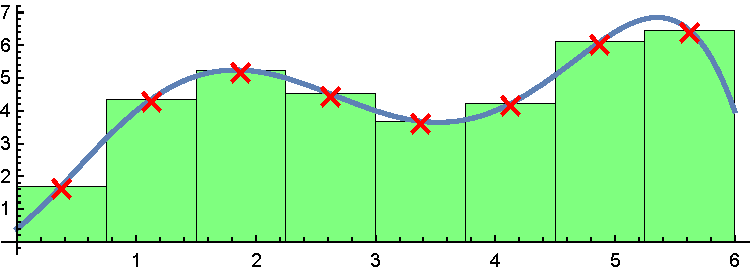
\includegraphics[width=0.7\textwidth]{images/midpoint-riemann.pdf}
\caption{A midpoint Riemann sum approximation.}
\label{fig:midpoint}
\end{figure}
If we replace the piece-wise constant approximation by a piece-wise linear approximation we get a \emph{trapezoidal rule approximation}. This approximation, illustrated in \fig{fig:trapezoidal}, is
\[ \int_a^b f(x) \dd x \approx \sum_{i=1}^{n-1} \frac{ f(x_i) + f(x_{i+1}) }{2} h \,. \]

\begin{figure}[H]
\centering
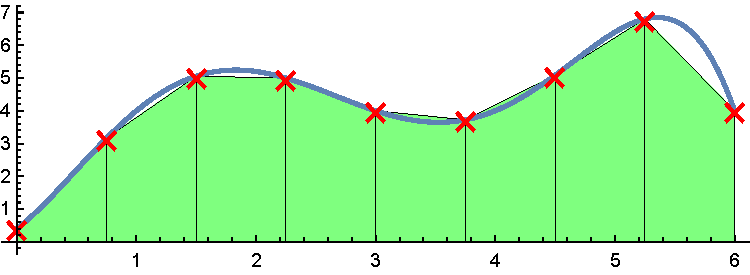
\includegraphics[width=0.7\textwidth]{images/trapezoidal.pdf}
\caption{A trapezoidal rule approximation.}
\label{fig:trapezoidal}
\end{figure}

This integration scheme may seem to be too simple to ever be used, but it will appear in Section~\ref{sec:laplace_inversion} on Laplace transform inversion. Trapezoidal integration has the property that it performs well on highly oscillatory integrands, such as integrals involving the complex exponential function.

The process can continue, with the approximations becoming higher order polynomials which interpolate the integrand. For example, if we split the range of integration as
\[ \int_a^b f(x) \dd x = \int_{x_1}^{x_3} f(x) \dd x + \int_{x_3}^{x_5} f(x) \dd x + \dots + \int_{x_{n-2}}^{x_n} f(x) \dd x \,, \]
then we can approximately integrate $\int_{x_1}^{x_3} f(x) \dd x$ by fitting a quadratic to the triplet \[ \bigl\{ \bigl( x_1, f(x_1) \bigr), \bigl(x_2, f(x_2)\bigr), \bigl(x_3, f(x_3)\bigr) \bigr\} \]
and integrating the resulting fit. This is called a \emph{Simpson's rule approximation}, and is illustrated in \fig{fig:simpson}.

\begin{figure}[H]
\centering
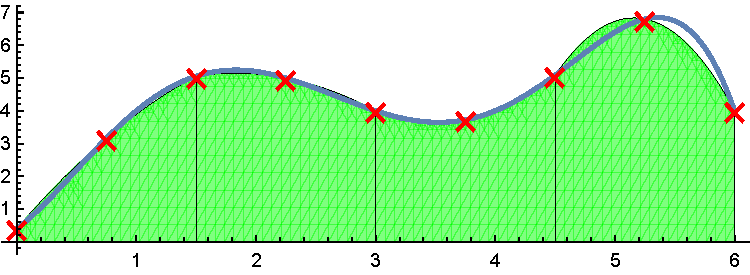
\includegraphics[width=0.7\textwidth]{images/simpson.pdf}
\caption{A Simpson rule approximation.}
\label{fig:simpson}
\end{figure}

The \emph{Newton--Cotes method} is the general case of this polynomial approximation.
Before elaborating, let us rewrite the problem to be the evaluation of $\int_a^b f(x) w(x) \dd x$ where $w(x)$ is called a \emph{weight function}.
The Newton--Cotes method approximates this integral as
\begin{equation} \label{NewtonCotesApprox}
\int_a^b f(x) w(x) \dd x \approx \int_a^b p_{n-1}(f; x_1, \dots, x_n; x) w(x) \dd x
\end{equation}
where $p_{n-1}(f; x_1, \dots, x_n; x)$ is the unique polynomial of degree $n-1$ which interpolates $f$ on the points $\{ x_1, \dots, x_n\}$ evaluated at the point $x$.
This interpolating polynomial, written in \emph{Lagrangian form}, is
\[ p_{n-1}(f; x_1, \dots, x_n; x) = \sum_{k=1}^{n} f(x_k) \ell_k(x) \,, \quad \text{where} \quad \ell_k(x) = \prod_{i=1, i\not=k}^n \frac{x - x_i}{x_k - x_i}  \,. \]
The approximating integral can be written as
\[ \int_a^b p_{n-1}(f; x_1, \dots, x_n; x) w(x) \dd x = \sum_{k=1}^n w_k f(x_k) \,, \]
where
\begin{equation} \label{NewtonCotesWeights}
	w_k = \int_a^b \ell_k(x) w(x) \dd x \qquad \text{for } k=1,\dots,n \,.
\end{equation}
For many common choices of weight function $w(x)$ (e.g.\ $w(x) = \e^{-x^2}$) and evaluation points $\{x_1,\dots,x_n\}$ (e.g.\ the constant step-size grid over $[-1,1]$, $x_i = -1 + 2 \frac{i-1}{n-1}$) these constants $w_k$ are available in the literature or in software packages.

For an arbitrary choice of $\{x_1, \dots, x_n\}$, the Newton--Cotes method has a surprising guarantee, which is that it will be exact when $f$ is a polynomial of degree $n-1$ or less. This is because the polynomial approximation of $f$ is just the original function $f$, i.e. $p_{n-1}(f; x_1, \dots, x_n; x) = f(x)$, so the $\approx$ becomes $=$ in \eqref{NewtonCotesApprox}. The name for this property is that the Newton--Cotes method with $n$ points has \emph{degree of exactness} $n-1$, and the natural next question is, can we achieve a greater degree of exactness than $n-1$ with just $n$ points?

We cannot achieve this. Specifically, we cannot do so by letting $\{x_1, \dots, x_n\}$ be an arbitrary choice. If we consider the form of the approximation
\begin{equation} \label{QuadratureGenForm}
	\int_a^b f(x) w(x) \dd x \approx \sum_{i=1}^n w_i f(x_i) \,,
\end{equation}
we can see that there are $2n$ free variables (the $x_i$ and the $w_i$) and only by choosing all $2n$ correctly we can achieve a degree of exactness of $2n-1$. The resulting approximation is called a \emph{Gaussian quadrature}, and its construction is based on the following theorem. First, we define the \emph{node polynomial} to be
\begin{equation} \label{NodePolynomial}
	\omega_n(x) = \prod_{k=1}^n (x - x_k) \,.
\end{equation}

\begin{theorem} \label{thm:GaussianQuadrature}
The approximation \eqref{QuadratureGenForm} will have degree of exactness of $2n -1$ iff:
\begin{enumerate}
\item the $w_k$ are given by \eqref{NewtonCotesWeights},
\item and the node polynomial $\omega_n(x)$ satisfies, for every polynomial $q$ of order $\le n-1$,
\begin{equation} \label{NodePolynomialOrthogonal}
	\int_{a}^b q(x) \omega_n(x) w(x) \dd x = 0  \,.
\end{equation}
\end{enumerate}
\end{theorem}

\begin{proof}
We only prove the $\Leftarrow$ direction. For the full proof (which the following is based on), see Theorem~3.2.1.\ of \cite{gautschi2011numerical}.

We wish to show that, for $f$ which is a polynomial of degree $2n-1$ or less,
\[ \int_a^b f(x) w(x) \dd x = \sum_{i=1}^n w_i f(x_i) \,. \]
Divide $f$ by $\omega_n$, so
\begin{equation} \label{PolynomialDivision}
	f(x) = q(x) \omega_n(x) + r(x)
\end{equation}
where the quotient $q$ and the remainder $r$ are polynomials of order $\le n-1$, so
\[ \int_a^b f(x) w(x) \dd x = \int_a^b q(x) \omega_n(x) w(x) \dd x + \int_a^b r(x) w(x) \dd x \,. \]
The first integral on the right-hand side is zero by \eqref{NodePolynomialOrthogonal},
and since $r$ is of order $\le n-1$, we know its $n$-point Newton--Cotes approximation is exact, i.e.
\[ \int_a^b r(x) w(x) \dd x = \sum_{i=1}^n w_i r(x_i) \,, \]
so rearranging \eqref{PolynomialDivision} gives
\[ \int_a^b f(x) w(x) \dd x = \sum_{i=1}^n w_i r(x_i) = \sum_{i=1}^n w_i [f(x_i) - q(x_k) \omega_n(x_k)] = \sum_{i=1}^n w_i f(x_i) \,. \]
\end{proof}

Finding the precise $\{x_1, \dots, x_n\}$ which satisfy the requirements of \thrm{thm:GaussianQuadrature} is easier than it seems. Equation \eqref{NodePolynomial} shows us that we just need to set $\{x_1, \dots, x_n\}$ to be the zeros of the node polynomial, and the second condition \eqref{NodePolynomialOrthogonal} tells us that the node polynomial $\omega_n(x)$ is the $n$-th orthogonal polynomial with respect to the weight function $w(x)$ over $[a,b]$.

So, the procedure for Gaussian quadrature is to find the $n$-th orthogonal polynomial for the given weight function $w(x)$ and range of integration $[a,b]$ (either by looking in the literature or by Gram--Schmidt orthogonalisation), set $\{x_1, \dots, x_n\}$ to be zeros of this polynomial, and set the $w_k$ by \eqref{NewtonCotesWeights}.

There is a large literature on quadrature (cf.\ \cite{gautschi2011numerical} and references), however these algorithms are subject to the ominously-named \emph{curse of dimensionality}. This phrase refers to the fact that, when trying to achieve some fixed accuracy using the approximation
\begin{equation*} \label{basic_num_int}
\Exp[g(\bfX)] \approx \sum_{i=1}^n w_i g( \bfx_i ) f_{\bfX}( \bfx_i ) \,,
\end{equation*}
the number of evaluation points $n$ required increases exponentially in the dimension $d$. Thus, the rule of thumb is to use quadrature with caution for $d$ in the range of about 1--5, and consider other approaches for larger $d$ (unless the integrand is particularly smooth).


\subsection{Laplace transform inversion} \label{sec:laplace_inversion}

To discuss Laplace transform inversion, we must first define the Laplace transform.

\begin{definition} \label{def:TransformDefs} For a function $f : \RL_+ \to \RL_+$, we define
\[
	\LT{f}(t) \defeq \int_{0}^{\infty} \e^{-t x} f(x) \dd x\,, \quad \text{for } t \in \CL \text{ with } \Re(t) \ge 0 \,, \\
\]
to be the corresponding \emph{Laplace transform}.
For a positive random variable $X$ with probability density function (pdf) $f_X$, we write $\LTsub{X}(t) \defeq \LT{f_X}(t) = \Exp[\e^{-tX}]$. \hfill $\diamond$
\end{definition}
Some useful relations for Laplace transforms include, for $t>0$
\[ \LT{ F_X }(t) = \frac{\LT{f_X}(t)}{t} = \frac{\LTsub{X}(t)}{t} \,, \text{ and } \]
\[ \LT{ \Ftail_X }(t) = \frac1t - \LT{F_X(x) }(t) = \frac{1 - \LTsub{X}(t)}{t}  \,. \]

A function $f$ can be recovered from its Laplace transform by a standard Bromwich integral.
We assume $f:\,\RL_+ \to \RL_+$, is a measurable function with locally bounded variation.
To define the Bromwich integral, first select a $\gamma > 0$ then
\[
f(x)=\frac{2\e^{\gamma x}}{\pi}\int_{0}^{\infty}\cos(xs)\Re\left[\LT{f}(\gamma + \ih s)\right]\dd s.
\]
We apply a basic quadrature rule to the Bromwich integral by first \emph{discretizing} the integral and then \emph{truncating} the resulting infinite sum. In both steps, we follow the steps of Abate and Whitt \cite{Abate1992}.

\subsubsection{Discretisation} \label{Sub:Discretization}

We will use a semi-infinite trapezoidal rule, despite the apparent simplicity of the method.
With a grid size $h>0$, this discretisation yields
\[
f(x) \approx f_{\mathrm{disc}}(x) \defeq \frac{2\e^{\gamma x}}{\pi} \cdot h \, \bigl \{ \tfrac12 \LT{f}(\gamma) + \sum_{j=1}^\infty  \cos(x \cdot hj)\Re\left[\LT{f}(\gamma + \ih hj)\right] \bigr \},
\]
since  $\Re\left[\LT{f}(\gamma)\right] = \LT{f}(\gamma)$. We simplify this by choosing $h = \pi/(2 x)$ and $\gamma = a / (2 x)$ for an $a > 0$, achieving
\begin{equation} \label{DiscretizedInversion}
f_{\mathrm{disc}}(x) = \frac{\e^{a/2}}{2x}\LT{f} \left(\frac{a}{2 x}\right) + \frac{\e^{a/2}}{x} \sum_{k=1}^\infty (-1)^{k} \Re\left[\LT{f}\left(\frac{a+ 2\pi \ih k}{2 x}\right)\right] \,.
\end{equation}

From Theorem~5.5.1 of \cite{RoScScTe08} we have that the \emph{discretisation error} (also called \emph{sampling error}) is simply
\begin{equation} \label{DiscretizationError}
    f_{\mathrm{disc}}(x) - f(x) = \sum_{k=1}^\infty \e^{-a k} f[ (2k+1) x ] \,.
\end{equation}
In particular, if $0 \le f(x) \le 1$, then
\begin{equation} \label{BoundedDiscretizationError}
    f_{\mathrm{disc}}(x) - f(x) \le \frac{\e^{-a}}{1-\e^{-a}} \,.
\end{equation}

There are no absolute value signs here --- the discretisation introduces a systematic overestimate of the true value.
Also, \eqref{DiscretizationError} implies $a$ should be as large as possible (limited eventually by finite-precision computation).
The benefit of knowing this result is slightly offset by the requirement that $h$ and $\gamma$ now be functions of $x$ rather than constants.

\subsubsection{Truncation}

Due to the infinite series, the expression in \eqref{DiscretizedInversion} cannot be directly computed, thus it has to be truncated.
The arbitrary-seeming choice of $h$ and $\gamma$ in Section~\ref{Sub:Discretization} not only allows for calculation of the discretisation error, but also benefits the truncation step. This is because the sum in \eqref{DiscretizedInversion} is (nearly) of alternating sign, and thus \emph{Euler series acceleration} can be applied to decrease the truncation error. Define for $\ell=1,2,\dots$
\begin{equation*} \label{TruncatedInversion}
s_\ell(x) \defeq \frac{\e^{a/2}}{2x}\LT{f} \left(\frac{a}{2 x}\right) + \frac{\e^{a/2}}{x} \sum_{k=1}^\ell (-1)^{k} \Re\left[\LT{f}\left(\frac{a+ 2\pi \ih k}{2 x}\right)\right] \,.
\end{equation*}
Then, for some positive integers $M_1$ and $M_2$,
\begin{equation}\label{eq:FinalApproxLaplaceInversion}
f(x) \approx f_{\mathrm{disc}}(x) \approx f_{\mathrm{approx}}(x) \defeq \sum_{k=0}^{M_1} \binom{M_1}{k} 2^{-M_1} s_{M_2+k}(x) \,.
\end{equation}

\subsection{Orthogonal polynomials} \label{subsc:ortho_poly}

We begin by a discussion of orthogonality of functions and generalised Fourier series expansions. This exposition draws on \cite{Szegoe1939} and \cite{gautschi2011numerical}. Firstly, we will define some vector space notation for a space over $\RL$ with respect to a \emph{weight function} $w : \RL \to \RL_+$. For the purposes of this thesis, we have that $w$ is a pdf, i.e.\ $\int_{\RL} w(x) \dd x = 1$.

\begin{definition}
We define the weighted inner product of functions $f$ and $g$ to be
\[ \langle f, g \rangle_w \defeq \int_{\RL} f(x) g(x) w(x) \dd x \]
and say that a function's weighted 2-norm is
\[ \norm{f}_w \defeq \sqrt{\langle f, f \rangle_w} \,. \]
This defines a vector space we denote $\Lp^2(\RL, w(x) \dd x)$, where $f \in \Lp^2(\RL, w(x) \dd x)$ means that $\norm{f}_w < \infty$.
\end{definition}

\begin{definition}
We say the functions $f_1, \dots f_n \in \Lp^2(\RL, w(x) \dd x)$ are \emph{linearly independent} if an affine combination of the functions is zero only if all coefficients are zero, i.e.
\[ \sum_{i=1}^n c_i f_i \equiv 0 \Rightarrow c_1 = \dots = c_n = 0\,. \]
\end{definition}

\begin{definition} \label{def:orthogonal}
We say a set of functions $\phi_1, \dots \phi_n \in \Lp^2(\RL, w(x) \dd x)$ are \emph{orthogonal} if
\begin{equation} \label{orthogonality}
\langle \phi_i, \phi_j \rangle_w = \int_{\RL} \phi_i(x) \phi_j(x) w(x) \dd x =
\begin{cases}
	0 & i \not=j \\
	c_i & i = j
\end{cases} \,.
\end{equation}
If the $c_i$ are all equal to 1, then we say the functions are \emph{orthonormal}. If not, one can construct \emph{normalised} versions of them, $\overline{\phi}_i(x) = \phi_i(x)/\norm{\phi_i}_w$, which are orthonormal.
\end{definition}

Any set of linearly independent functions can be used to construct a set of orthogonal functions (and hence a set of orthonormal functions), a process which is called \emph{orthogonalisation}. Algorithm~\ref{alg:gs} shows the well-known \emph{Gram--Schmidt} procedure for orthogonalisation.

\begin{algorithm}
\caption{Gram--Schmidt orthogonalisation}
\label{alg:gs}
\begin{algorithmic}[1]
\Function{Gram--Schmidt}{$f_1$,\dots,$f_n$, $w$}
\For{$i \gets 0, \dots, n$}
\State $\phi_i \gets f_i$
\For{$j = 0, \dots, i-1$}
\State $\phi_i \gets \phi_i - \langle f_i, \phi_j \rangle_w \phi_j$
\EndFor
\State $\overline{\phi}_i \gets \phi_i / \norm{\phi_i}_w$
\EndFor
\State \textbf{return} $\{ \overline{\phi}_0, \dots, \overline{\phi}_n \}$
\EndFunction
\end{algorithmic}
\end{algorithm}



\begin{definition}
Given a family of orthonormal functions $\phi_0, \phi_1,\dots \in \Lp^2(\RL, w(x) \dd x)$, and some real function $f$, we define the \emph{generalised Fourier expansion} of $f$ to be $\sum_{i=0}^\infty f_i \phi_i(x)$ where the Fourier coefficients are $f_i = \langle f, \phi_i \rangle_w$.
\end{definition}

The following theorem (adapted from Theorem~2.1.2 of \cite{Szegoe1939}) considers how Fourier expansions perform as function approximations:

\begin{theorem}
Given $f \in \Lp^2(\RL, w(x) \dd x)$ and the orthonormal functions $\phi_0,\dots,\phi_n$, consider all functions of the form $g_n(x) = \sum_{i=0}^n c_i \phi_i(x)$. The specific $g_n$ which minimises $\norm{f - g_n}_w$, equivalently which minimises $\norm{f - g_n}_w^2$, is $g_n^* = \sum_{i=0}^n f_i \phi_i = \sum_{i=0}^n \langle f, \phi_i \rangle_w \phi_i$.
\end{theorem}
\begin{proof}
We minimise the error by setting the derivative to zero; the resulting stationary point will be the unique minimiser of the error since it is of quadratic form. The error is
\begin{align*}
\norm{f - g_n}_w^2 &= \langle f-g_n, f-g_n \rangle_w = \norm{f}_w^2 -2 \langle f, g_n \rangle_w + \norm{g_n}_w^2 \\
&= \norm{f}_w^2 - 2 \int_{\RL} f(x) [\sum_{i=0}^n c_i \phi_i(x) ] w(x) \dd x + \int_{\RL} \sum_{i,j=0}^n c_i c_j \phi_i(x) \phi_j(x) w(x) \dd x \,.
\end{align*}
Taking derivatives inside the integrals yields
\begin{align*}
\frac{\dd \norm{f - g_n}_w^2}{\dd c_k}
&= \int_{\RL} \sum_{i=0}^n 2 c_i \phi_i(x) \phi_k(x) w(x) \dd x - 2 \int_{\RL} f(x) \phi_k(x)  w(x) \dd x \\
&= 2 \bigl[ \sum_{i=0}^n  c_i \langle \phi_i, \phi_k \rangle_w - \langle f, \phi_k \rangle_w \bigr] = 2 \bigl[ c_k - \langle f, \phi_k \rangle_w \bigr]
\end{align*}
where the last equality follows from the orthonormality of the $\phi_i$. Setting each derivate to zero, $\frac{\dd}{\dd c_k} \norm{f - g_n}_w^2 \equiv 0$, yields the stated minimiser as $c_k = \langle f, \phi_k \rangle_w$.
\end{proof}

This theorem motivates using approximations of the form $g_n^*(x) \defeq \sum_{i=0}^n \langle f, \phi_i \rangle_w \phi_i(x)$. The error for the $g_n^*$ approximation is
\begin{equation*} \label{ortho_error}
\norm{f - \sum_{i=1}^n f_i \phi_i}_w^2 = \int_{\RL} f(x)^2 w(x) \dd x - \sum_{i=1}^n f_i^2 = \norm{f}_w^2 - \sum_{i=1}^n f_i^2 \,.
\end{equation*}
From this, we can see that increasing $n$ will not increase the error, so the sequence of non-negative errors
\begin{equation*} \label{error_sequence}
\norm{f - g_1^*}_w^2 \ge \norm{f - g_2^*}_w^2 \ge \norm{f - g_3^*}_w^2 \ge  \dots
\end{equation*}
must converge to a limiting value. It is desirable for this limit to be 0.

\begin{definition}
If for every $f \in \Lp^2(\RL, w(x) \dd x)$, with $g_n^* = \sum_{i=1}^n \langle f, \phi_i \rangle_w \phi_i$, we satisfy $\norm{f - g_n^*}_w^2 \to 0$ as $n \to \infty$, we say that the orthonormal sequence $\{ \phi_i \}_{i \in \NZ}$ is \emph{complete} in $\Lp^2(\RL, w(x) \dd x)$.
\end{definition}

When we work with a complete orthonormal sequence $\{ \phi_i \}_{i \in \NZ}$, then for any function $f \in \Lp^2(\RL, w(x) \dd x)$ and $\epsilon > 0$, we can find an $N$ so that
\[ \norm{ f - g_N^* }_w^2 \le \epsilon \,. \]
We return to the question of completeness after first specifying the orthonormal sequences we will use.

Now, consider the case where the orthonormal sequence $\{ \phi_i \}_{i \in \NZ}$ are polynomials.

\begin{definition}
We say $\{ p_k \}_{k\in\NZ}$ are the orthonormal polynomials for $\Lp^2(\RL, w(x) \dd x)$ if: i) $p_k$ is a polynomial of order $k$, and ii) the polynomials are orthonormal as per Definition~\ref{def:orthogonal}.
\end{definition}

These can be constructed from the sequence $1, x, x^2, \dots$ of monomials. The monomials are linearly independent for all choices of $w$, so one can orthogonalise them by using the iterative Gram--Schmidt outlined in Algorithm~\ref{alg:gs}.

Alternatively, there exists a somewhat complicated direct method for constructing them. We denote the moments of the weight pdf as $m_i = \int_{\RL} x^i w(x) \dd x$, and construct Hankel matrices of them as
\[ \bfH_n = \begin{pmatrix}
m_0 & m_1 &  m_2 &\cdots & m_n \\
m_1 & m_2 &  m_3 &\cdots & m_{n+1} \\
&&\vdots&& \\
m_{n-1} &m_n& m_{n+1} &\cdots &m_{2n-1}\\
m_n &m_{n+1}& m_{n+2} &\cdots &m_{2n}
\end{pmatrix} \,, \quad n \in \NL \,. \]
Lastly, if we denote $\tilde{\bfH}_n(x)$ to be the Hankel matrix $\bfH_n$ where the last row is replaced by $(1, x, x^2, \dots, x^n)$, we can write
\begin{equation} \label{ortho_poly_gen_form}
p_n(x) = \frac{1}{\sqrt{ \det( \bfH_{n-1} ) \det( \bfH_n ) }} \det( \tilde{\bfH}_n(x) ) \,, \quad n \in \NL \,.
\end{equation}
For more details, see \cite[pp.\ 26--27]{Szegoe1939}.
This method is performed in Appendix~\ref{app:lognormal_poly} to describe the orthonormal polynomials w.r.t.\ the pdf of a lognormal distribution.


For orthonormal polynomial systems, there is a simple condition on the weight function $w$ which implies completeness:
\begin{proposition} \label{prop:complete_polynomials}
If there exists an $\alpha>0$ such that
\begin{equation*}
\int_{\RL} \e^{\alpha|x|} w(x) \dd x < \infty\,,
\end{equation*}
then the orthonormal polynomials $\{ p_k \}_{k\in\NZ}$ are complete in $\Lp^2(\RL, w(x) \dd x)$.
\end{proposition}

See \cite[p.\ 333]{Na65} for the proof.


\subsection{Monte Carlo techniques} \label{sec:monte_carlo_integration}

When analytic integration and quadrature both fail, we can attempt \emph{Monte Carlo integration (MCI)}. Say we want to estimate $\ell = \Exp[ g(\bfX) ]$. If we can sample values $R \in \NL$ independent and identically distributed (iid) vectors from the distribution $f_{\bfX}$, denoted $\bfX^{[r]} \iidDist f_{\bfX}$, then we have the \emph{crude Monte Carlo (CMC)} estimator
\begin{equation} \label{basic_mci}
\hat{\ell}_{\mathrm{CMC}} = \frac1R \sum_{r=1}^R g(\bfX^{[r]}) \,.
\end{equation}
The estimator is unbiased, meaning $\Exp[ \hat{\ell}_{\mathrm{CMC}} ] = \ell$, and by the law of large numbers we know $\hat{\ell}_{\mathrm{CMC}} \convas \ell$ as $R \to \infty$.

When $\sigma^2 \defeq \Var[ g(\bfX) ] < \infty$, the central limit theorem applies, so
\begin{equation} \label{mci_clt}
\sqrt{R} \, \hat{\ell}_{\mathrm{CMC}} \convdistr \NormDist(\ell, \sigma^2) \qquad \text{as } R \to \infty \,.
\end{equation}
If we choose $R$ to be large, then we can say $\sqrt{R} (\hat{\ell}_{\mathrm{CMC}} - \ell)/ \sigma \approxdistr \NormDist(0, 1)$ and generate approximate confidence intervals at significant level $\alpha \in (0,1)$,
\begin{equation} \label{CMC_CI}
\Prob\bigl( \ell - q_{1-\alpha/2} \frac{\sigma}{\sqrt{R}} \le \hat{\ell}_{\mathrm{CMC}} \le \ell + q_{1-\alpha/2} \frac{\sigma}{\sqrt{R}} \bigr) \approx 1 - \alpha \,.
\end{equation}
To actually evaluate this, we substitute the standard estimate $\hat{\sigma}$ for $\sigma$,
\begin{equation} \label{basic_mci_var}
\hat{\sigma}^2 = \frac1{R-1} \sum_{r=1}^R (g(\bfX^{[r]}) - \hat{\ell}_{\mathrm{CMC}})^2 \,.
\end{equation}
Alternatively, we could use bootstrapping to produce approximate confidence intervals without assuming that the asymptotic normality of $\hat{\ell}_{\mathrm{CMC}}$ has already kicked in.

Considering these confidence intervals, we can see this method allows us to escape the event-horizon of the curse of dimensionality. Increasing the accuracy of the estimator by 1 significant figure (for a fixed significance level $\alpha$) corresponds to increasing $R$ by a factor of 100, since \eqref{mci_clt} tells us the error is of order $\Oh(R^{-1/2})$. The amazing conclusion is that this factor of 100 is unaffected by the dimension $d$ of the integral $\ell$ which is being approximated.

What is also amazing is that increasing $R$ by 100, which is equivalent to increasing the computational burden by 100, is an enormous cost to pay for a paltry significant figure of accuracy. We return to this problem later when we discuss quasi-Monte Carlo.

Next, we consider the common algorithms for generating random variables from a specified distribution, then consider \emph{variance reduction techniques} which can greatly improve the efficiency of the Monte Carlo method.

\subsubsection{Sampling uniforms}

Sampling from any probability distribution relies upon a sequence of random numbers from the $\UnifDist(0,1)$ distribution. Typically, we do not use truly random numbers, but pseudorandom numbers which mimic the behaviour of uniform random variables. This means that the $n$-th pseudorandom number $u_n$ is a deterministic function of the previous $u_{n-1}$; cf.\ Chapter 1 of \cite{kroese2013handbook} for more on pseudorandom number generation, and the famous generator called the \emph{Mersenne twister}.

\subsubsection{Inverse transform method}

Say that we want to generate $X^{[r]} \iidDist f_X$, we can set
\[ X^{[r]} = F_X^{\ginv}(U^{[r]}) \text{ where } U^{[r]} \iidDist \UnifDist(0,1) \,, \]
where $F_X^{\ginv}(u)$ is the (quasi-)inverse
$ F_X^{\ginv}(u) \defeq \inf \{ x : F_X(x) \ge u \}  $ for $0 \le u \le 1$.
How can we evaluate $F_X^{\ginv}$? It is sometimes known analytically, the canonical example being $X \sim \ExpDist(\lambda)$, so $F_X(x)=1 - \e^{-\lambda x}$, and hence $F^{\ginv}(u) = -\log(1-u)/\lambda$.

In most other cases, we need to perform a root-finding step, for example using the Newton--Raphson method, to invert $F_X$ approximately. If we cannot even (analytically) integrate the pdf $f_X$ to find the cdf $F_X$, then this method is almost hopeless. Similarly, if we only know $f_X$ up to a constant of proportionality, or if we want to simulate $d>1$ dimensions, then we must turn to other methods.

One useful aspect of the inverse transform method is that it allows one to simulate $X$ conditional on $X > \gamma$, by
\[ X^{[r]} = F_X^{\ginv}(\tilde{U}^{[r]}) \text{ where } \tilde{U}^{[r]} \iidDist \UnifDist( F_X(\gamma), 1 ) \,. \]
As $\gamma$ becomes very large ($\Prob(X > \gamma)$ becomes very small), then we are evaluating $F_X^{\ginv}$ near one. This can lead to numerical instability, so care must be taken that this technique does not return $X^{[r]} = \infty$ or $X^{[r]} = \mathrm{NaN}$.

\subsubsection{Acceptance--rejection}

Assume we have a distribution $f_Y$, called the \emph{proposal distribution}, and a $C > 0$ such that
\begin{equation} \label{ar-bound}
f_X(x) \le C f_Y(x) \quad \forall x \in \RL \,.
\end{equation}
If we can sample from the proposal distribution, then we can sample $f_X$ by Algorithm~\ref{alg:ar}.

\begin{algorithm}[H]
\caption{Acceptance--rejection}
\label{alg:ar}
\begin{algorithmic}[1]
\Function{Acceptance--rejection}{$f_X$, $f_Y$, $C$}
\While{True}
\State $Y \sim f_Y$, $U \sim \UnifDist(0,1)$
\If{$U \le f_X( Y ) / C f_Y( Y )$}
\State \textbf{return} $Y$
\EndIf
\EndWhile
\EndFunction
\end{algorithmic}
\end{algorithm}

Acceptance--rejection is quite general, as it works if $f_X(x)$ is substituted for $\tilde{f}_X(x) \propto f_X(x)$ in \eqref{ar-bound} and \alg{alg:ar}. \fig{fig:ar} illustrates an example of this.

\begin{figure}[H]
\centering
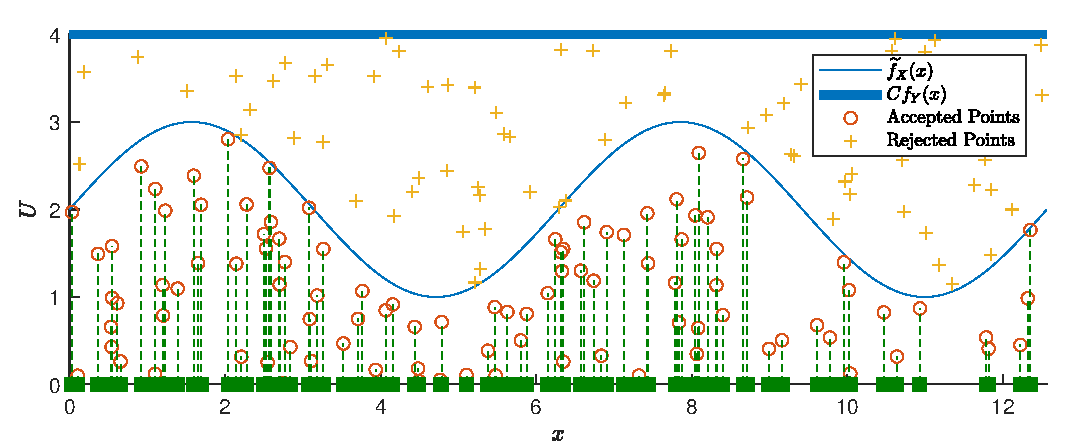
\includegraphics[width=0.95\textwidth]{images/ar.pdf}
\caption{Acceptance--rejection sampling from $\tilde{f}_X(x) = 2 + \sin(x)$ for $x \in [0, 4\pi]$ using the proposal distribution $\UnifDist[0,4\pi]$, $C=16\pi$, and sampling $R=100$ random variables.}
\label{fig:ar}
\end{figure}

This efficiency of acceptance--rejection depends heavily upon the constant $C$. If we use $f_X$ and not $\tilde{f}_X$ above (i.e.\ we know the normalising constant of the desired distribution) then $C$ can be easily interpreted. That is, the expected number of samples from $f_Y$ needed to accept one sample from $f_X$ is $1 / C$. So the optimal value of $C$ is 1; then, we never generate proposal samples which are wastefully discarded.

Determining $C$ can be laboriously done by hand, or it can be the result of a root-finding algorithm. Extending to $d>1$ dimensions is possible, but the determination of $C$ becomes even more difficult.

\subsubsection{Markov chain Monte Carlo}

The most general, and most complicated, form of sampling is \emph{Markov chain Monte Carlo (MCMC)}. While the algorithms listed above sample exactly from the desired target distribution $f_X$, MCMC samples will only be approximately from this distribution. Furthermore, the samples produced will not be independent and will not be identically distributed.

The main idea is to construct a Markov chain, $\{ X_n \}_{n\in\NZ}$, which has a stationary distribution which is equal to the target distribution $f_X$, then the LLN and the CLT both apply to the sequence $\frac1j\sum_{i=0}^j g(X_j)$. We will skip the Markov chain details as they are not relevant to this thesis, cf. \cite{meyn2012markov}, or for a general treatment on MCMC see any detailed textbook on Monte Carlo such as \cite{asmussen2007stochastic,glasserman2003monte,kroese2013handbook}.

The crucial step is to provide a \emph{transition kernel} $q(x \hookrightarrow y)$, which for every fixed $x$ in the support of $f_X$ is a pdf in $y$, i.e.\ $q(x \hookrightarrow \argdot) \ge 0$, and $\int_{\RL} q(x \hookrightarrow y) \dd y = 1$. Also, we need to be able to simulate from $q(x \hookrightarrow \argdot)$. If this is satisfied, then sampling becomes a sequence of \emph{Metropolis--Hasting} steps:

\begin{algorithm}
\caption{Markov chain Monte Carlo}
\label{alg:mcmc}
\begin{algorithmic}[1]
\Function{MCMC}{$f_X$, $R$, $q$, $X_0$}
\For{$r = 1$ to $R$}
\State $X_r^\ast \sim q(X_{r-1} \hookrightarrow \argdot)$
\State $U \sim \UnifDist(0,1)$
\If{$U \le [ f_X(X_r^\ast) q(X_r^\ast \hookrightarrow X_{r-1}) ] / [ f_X(X_{r-1}) q(X_{r-1} \hookrightarrow X_r^\ast) ] $}
\State $X_r \gets X_r^\ast$
\Else
\State $X_r \gets X_{r-1}$
\EndIf
\EndFor
\State \textbf{return} $(X_1, \dots, X_R)$
\EndFunction
\end{algorithmic}
\end{algorithm}

Sampling from a complicated distribution using MCMC can be more of an art than a science. The MCMC practitioner's toolbox includes a vast array of tricks: to assess whether the Markov chain has reached stationarity (often the samples from the start of the chain, called the \emph{burn in} period, are discarded), to see the effective number of samples (which is $\le R$, considering that many samples will be duplicated), to choose the arbitrary starting point(s) $X_0$ (it is common to run many chains from multiple starting points).

As alluded to earlier, the most important choice for the MCMC practitioner is to set the transition kernel. Being supplied \alg{alg:mcmc} without a specific transition kernel, is like being given a car without an engine. The MCMC literature supplies a baffling array of kernel options, each with varying degrees of hyperparameters which may need tuning. Modern MCMC research and software tools have thankfully moved in the direction of automatically choosing a good transition kernel, either by allowing the transition kernel to adapt to the target function $f_X$ while MCMC is in progress (called adaptive methods), or by using a technique called Hamiltonian MCMC.

MCMC is increasingly the only possible option for evaluating high-dimensional complicated integrals, especially if they are fit into the framework of Bayesian statistics. Yet if of the other integration techniques mentioned in this chapter were able to be used instead of MCMC, then they almost certainly should be used. In this sense, MCMC is the worst form of integration, except for all the others.


\subsubsection{Common random numbers}

We now turn to the problem of variance reduction. Consider the case where we have a Monte Carlo estimator $\hat{f}$ of a pdf $f$, and we wish to estimate this density at many points, $\hat{f}(x_1) \approx f(x_1), \dots, \hat{f}(x_n) \approx f(x_n)$. In this case, we can treat each problem separately, using $R$ random variables to construct an estimator $\hat{f}(x_1)$ then another $R$ random variables to construct $\hat{f}(x_2)$, and so on. Alternatively, we can generate $R$ random variables and share these between all $n$ estimation problems. This is called using \emph{common random numbers (CRN)}.

This produces a smoothing effect, illustrated by \fig{fig:crn} where the pdf of the sum of thirty iid $\GammaDist(3,2)$ random variables is estimated with and without CRN using the Monte Carlo estimator in \cite{Pushout}.\footnote{This is a toy problem as the sum is Erlang distributed.} While using CRN creates a more realistic result for miniminal effort, the effect diminishes as $R$ becomes larger.

\begin{figure}[H]
\centering
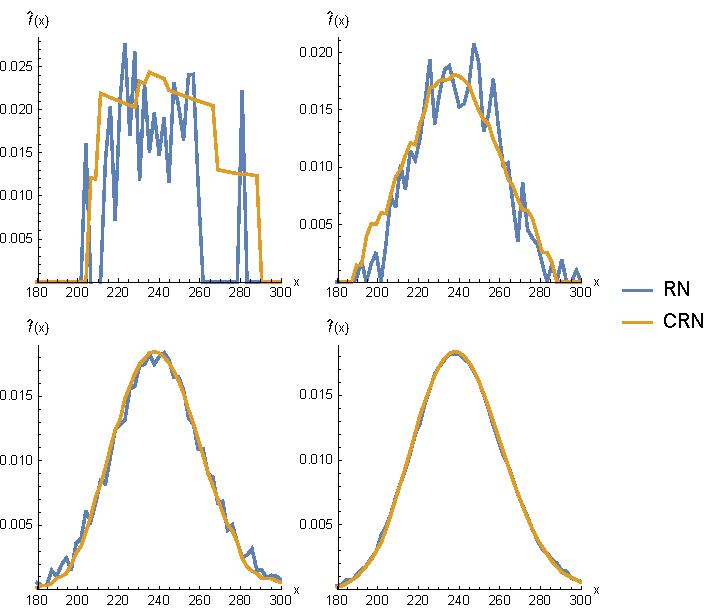
\includegraphics[width=0.75\textwidth]{images/crn.pdf}
\caption{Estimating a pdf with and without CRN, for $R = 10$, $10^2$, $10^3$, $10^4$ resp.}
\label{fig:crn}
\end{figure}

\subsubsection{Importance sampling}

One of the most useful variance reduction techniques follows from the old trick of multiplying by one. The expectation being evaluated, as an integral, is
\[ \ell = \Exp[ g(X) ] = \int_\RL g(x) f_X(x) \dd x = \int_{\RL} g(x) f_X(x) \frac{f_Y(x)}{f_Y(x)} \dd x = \Exp[ g(Y) \frac{f_X(Y)}{f_Y(Y)} ] \]
where $X \sim f_X$ and $Y \sim f_Y$, and so the \emph{importance sampling (IS)} Monte Carlo estimator is
\[ \hat{\ell}_{\mathrm{IS}} = \frac1R \sum_{r=1}^R g(Y^{[r]}) \frac{f_X(Y^{[r]})}{f_Y(Y^{[r]})} \,, \quad \text{for } Y^{[r]} \iidDist f_Y \,. \]
This approach holds so long as there are $x$ where $f_Y(x)=0$ but $f_X(x) > 0$, or in words, the support of $Y$ includes the support of $X$ (the jargon for this is that $f_X$ is absolutely continuous w.r.t.\ $f_Y$). The pdf $f_Y$ is called the \emph{proposal density}, and the fraction $f_X(Y) / f_Y(Y)$ is called the \emph{likelihood ratio} (or the Radon--Nikod{\'y}m derivative) and can be seen as correcting for the fact that we have changed the distribution which we are sampling from.

It is slightly misleading to call this technique a variance reduction algorithm, since with a poor choice of proposal pdf we can easily create estimators with \emph{more variance} than CMC. Yet for a well-chosen density, the variance reduction can be many orders of magnitude.

A well-known fact of importance sampling for estimating $\ell~=~\Prob(X~<~x)$ is that
\[ f_Y(x) = \frac{\ind{ X < x }}{\Prob(X < x)} f_X(x) \]
is the proposal density which minimises the variance of $\hat{\ell}_{\mathrm{IS}}$. It is easy to see that this proposal yields an unbiased estimator (all IS estimators are unbiased) which has zero variance!
\[ \hat{\ell}_{\mathrm{IS}} = \frac1R \sum_{r=1}^R \ind{ Y^{[r]} < x } \frac{f_X(Y^{[r]})}{ \frac{\ind{ Y^{[r]} < x }}{\Prob(X<x)} f_X(Y^{[r]})} = \frac1R \sum_{r=1}^R \Prob(X<x) = \ell \,. \]
Obviously the result is without immediate practical value, since to create this proposal density we need to normalise by the unknown probability which is being estimated in the first place. However, it does provide the intuition for selecting proposal densities: choose proposals which increases the probability of interesting events.

If the problem is to estimate $\ell = \Prob(X > \gamma)$ for a large $\gamma$, then proposals should be taken which increase the probability of large samples. One scheme, called \emph{exponential tilting} (or \emph{twisting}), is frequently used, in which
\begin{equation} \label{def-exp-tilting}
f_Y(x) = \frac{\e^{\theta x}}{\Exp[\e^{\theta X}]} f_X(x)
\end{equation}
where $\theta$ is a positive constant (it can be negative if we wish to induce more small samples). The optimal choice of $\theta$ can be calculated, and it is the value which satisfies $\Exp[Y] = \gamma$.

Exponential tilting (with a positive $\theta$) is only applicable when the original distribution $f_X$ has a well-defined moment generating function (otherwise $\Exp[\e^{\theta X}] = \infty$). A similar technique which can be employed (if $X$ is a positive random variable) in this scenario is \emph{hazard rate twisting},
\[ f_Y(x) = (1-\theta) f_X(x) \e^{\theta \Lambda_X(x)} \]
in which $\Lambda_X(x) = \int_0^x \lambda_X(x) \dd x$ where $\lambda_X$ is the hazard rate of $X$, i.e., the ratio of its pdf to its survival function \cite{juneja2002simulating}.

One limitation for any IS scheme is that the proposal density must be chosen to reduce variance, but must also allow us to simulate from it. Luckily there are many cases where the exponentially-tilted pdf describes a distribution within the same family as the original pdf (this is true for distributions in the \emph{natural exponential family}, including the normal, gamma, Poisson and Weibull distributions), and so the difficulty in simulation is not increased over CMC.

\subsubsection{Conditional Monte Carlo}

Sometimes we can introduce extra theoretical knowledge to a Monte Carlo problem to decrease the variance. This is the main idea of \emph{conditional Monte Carlo}, in which we simplify certain problems by using properties of conditional probability. This is easiest seen with an example: say we wish to estimate $\ell = \Prob(X_1 + X_2 > \gamma)$, then the CMC estimator is
\[ \hat{\ell}_{\mathrm{CMC}} = \frac1R \sum_{r=1}^R \ind{ X_1^{[r]} + X_2^{[r]} > \gamma } \,,\quad (X_1,X_2) \iidDist F_{\bfX} \,. \]
Yet we also know that $\Prob(X_1 + X_2 > \gamma \mid X_2 = x_2) = \Prob(X_1 > \gamma - x_2) = \Ftail_{X_1}(\gamma - x_2)$, which motivates a conditional MC estimator
\[ \hat{\ell}_{\mathrm{Cond}} = \frac1R \sum_{r=1}^R \Ftail_{X_1}(\gamma - X_2^{[r]}) \,, \quad X_2 \iidDist F_{X_2} \,. \]
An advantage of conditional MC is that the variance will either decrease or stay the same relative to the CMC estimator. This technique can achieve a remarkable variance reduction, as exemplified by the Asmussen--Kroese estimator \cite{asmussen2006improved}; also, see \cite{asmussen2017conditional} for a recent review of conditional MC for sums of random variables.

\subsubsection{Quasi-Monte Carlo}

The main ingredient of CMC is randomness, and though we know that on average CMC's results are accurate, we can simply be unlucky and see an estimation which is very innaccurate. How does this happen, if for example, we are trying to estimate $\ell = \int_{[0,1]^d} f(\bfu) \dd u$ by $\hat{\ell} = \frac1R \sum_{r=1}^R f(\bfU^{[r]})$ for $\bfU^{[r]} \iidDist \UnifDist([0,1]^d)$? It can occur if the $\bfU^{[r]}$ cluster together, and the integrand's behaviour is not fully considered over its range $[0,1]^d$. This leads to the question, can we constrain the $\bfU^{[r]}$ so that they do not overly cluster together?

This reasoning leads us to \emph{quasi-Monte Carlo (QMC)}, where random $(\bfU^{[1]},\dots,\bfU^{[R]})$ sampling points are replaced by deterministic $(\bfu_1,\dots, \bfu_R)$ which are designed to be evenly spread across the $d$-dimensional hypercube. \fig{fig:qmc} shows scatterplots of 2 dimensional uniform points and from a QMC \emph{low-discrepency sequence} called Sobol's sequence.

\begin{figure}[H]
\centering
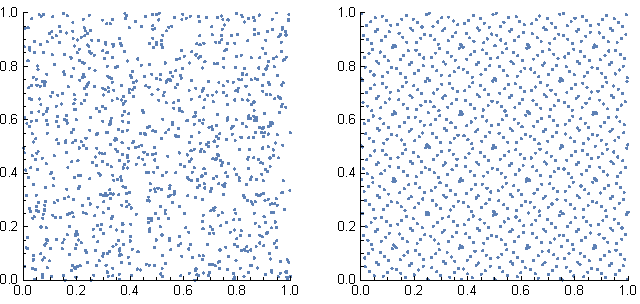
\includegraphics[width=0.8\textwidth]{images/qmc.pdf}
\caption{Scatterplot of $R=1024$ iid two-dimensional $\UnifDist(0,1)$ random variables, and 1024 points of the two-dimensional Sobol sequence resp.}
\label{fig:qmc}
\end{figure}

Designing and analysing new QMC schemes is a field of ongoing research, with a large active community. An allure of QMC is that there are bounds on the integration error, e.g.\ for a smooth integrand $f$ the \emph{Koksma--Hlawka inequality} \cite{asmussen2007stochastic,dick2010digital,glasserman2003monte} is
\[ \Bigl| \int_{[0,1]^d} f(\bfu) \dd \bfu - \frac1R \sum_{r=1}^R f(\bfu_r) \Bigr| \le V(f) D^\ast(\bfu_1,\dots,\bfu_R) \]
where $V(f)$ is the Hardy--Krause variation, and $D^\ast$ is the star discrepency $(\bfu_1,\dots, \bfu_R)$.

As $D^\ast(\bfu_1,\dots, \bfu_R) = \Oh( (\log R)^d / R ) = \Oh( R^{-(1-\epsilon)} )$ for all $\epsilon > 0$, we can see that QMC techniques offer an error which can be close to $\Oh(R^{-1})$. The comparable CMC error guarantee, arrived at by we rearranging the approximate confidence intervals result in \eqref{CMC_CI} is
\[ \Bigl| \int_{[0,1]^d} f(\bfu) \dd \bfu - \frac1R \sum_{r=1}^R f(\bfU^{[r]}) \Bigr| \le q_{1-\alpha/2} \frac{\sigma}{\sqrt{R}} \]
with probability $1-\alpha$. While the two statements are not directly comparable (the CMC claim is a probabilistic bound), it seems that for $R$ large enough QMC allows us to break out of unimpressive $\Oh(R^{-1/2})$ rate up to something approaching $\Oh(R^{-1})$, if the dimension of the problem is not too high.

\subsubsection{Rare events}

One common problem in financial and insurance applications is estimating the likelihood of rare events (e.g.\ market crashes, or extreme climate events). In this context, using CMC can be difficult. For example, let us say that we want to estimate $\ell(\gamma) = \Prob(X > \gamma)$ with
\begin{equation} \label{cmc_prob_est}
\hat{\ell}_{\mathrm{CMC}} = \frac1R \sum_{r=1}^R \ind{ X^{[r]} > \gamma) }
\quad \text{where } \bfX^{[r]} \iidDist f_X \,.
\end{equation}
If the true probability is $\ell(\gamma) = 10^{-10}$, and we set $R=10^6$ then about 99.99\% of the time we simply get the estimate $\hat{\ell}_{\mathrm{CMC}} = 0$. Since every indicator function returned 0, then the variance estimate for $\hat{\ell}_{\mathrm{CMC}}$ is also 0, and hence the confidence intervals are also $[0,0]$.

A simple solution to this problem is to employ importance sampling, though this can lead to likelihood degeneration for large enough $\gamma$. More complicated iterative methods can be employed, such as the \emph{cross-entropy method} \cite{de2005tutorial}, or \emph{multi-level splitting} \cite{glasserman1996splitting,glasserman1999multilevel,cerou2007adaptive}. These methods are similar to MCMC in that they require great care in choosing parameters and can significantly increase the computing time necessary to allow for the increased generality. For more details, see \cite{rubino2009rare} or \cite{kroese2013handbook}.

Given an IS estimator, we can categorise its rare-event performance into different categories.

\newpage
\begin{definition} An estimator $\hat{p}_{\gamma}$ of some rare probability $p_{\gamma}$ which satisfies $\forall \epsilon>0$ \\
\begin{subequations}
 \begin{tabularx}{\hsize}{XXX}
     \begin{equation*}
       \limsup\limits_{\gamma\to\infty} \, \frac{\Var\hat p_{\gamma}}
	{p_{\gamma}^{2-\epsilon}}=0
     \end{equation*} &
     \begin{equation*}
       \limsup\limits_{\gamma\to\infty}\frac{\Var \hat{p}_{\gamma}}
	{p_{\gamma}^2}<\infty
     \end{equation*} &
     \begin{equation*}
       \limsup\limits_{\gamma\to\infty} \, \frac{\Var\hat{p}_{\gamma}}{p_{\gamma}^2}=0
     \end{equation*}
   \end{tabularx}
\end{subequations}
has \emph{logarithmic efficiency}, \emph{bounded relative error}, or \emph{vanishing relative error} respectively. These are in increasing order of strength, that is,
\[ \text{Vanishing relative error} ~ \Rightarrow ~ \text{Bounded relative error} ~ \Rightarrow ~ \text{Logarithmic efficiency} \,. \]
\end{definition}

These allow us to compare two competing methods on their theoretical properties. Of course, just as the seemingly inefficient $\Oh(n^2)$ \emph{quicksort} algorithm is usually faster than the $\Oh(n \log n)$ \emph{mergesort} algorithm, the fact that an estimator satisfies vanishing relative error does not always translate into better variance reduction.

\subsection{Dependence and copulas}

A theme of modern probability research, and of this thesis, is to relax the independence assumptions which constrict older models. \emph{Copulas} allow us to analyse just the dependence structure of a random vector, without considerations of the marginal distributions. A copula is a joint cdf for a random vector of $\UnifDist(0,1)$ random variables. \emph{Sklar's theorem} which is shown below (adapted from \cite{nelsen2006introduction}) is the foundational result which shows the generality of copulas.

\begin{theorem}[Sklar's theorem]

Consider a random vector $\bfX=(X_1,X_2)$ which has the joint cdf $F_{\bfX}$ and marginal cdfs $F_{X_1}$ and $F_{X_2}$. We can write
\begin{equation} \label{copula_def}
F_{\bfX}(x_1, x_2) = C( F_{X_1}(x_1), F_{X_2}(x_2) )
\end{equation}
where $C$ is a copula, and if $F_{X_1}$ and $F_{X_2}$ are both continuous then $C$ is unique. Conversely, if $C$ is a copula, and $F_{X_1}$ and $F_{X_2}$ are cdfs, then the function $ C( F_{X_1}(\argdot), F_{X_2}(\argdot) )$ is a joint cdf with marginals $F_{X_1}$ and $F_{X_2}$.

\end{theorem}

The definition \eqref{copula_def} can be extended to any number of dimensions, and the definition can be reversed to get
\begin{equation} \label{cop_first}
C(u_1, \dots, u_d) = \Prob(X_1\le F_{X_1}^{{\ginv}}(u_1), \dots, X_d \le F_{X_d}^{\ginv}(u_d))  \,.
\end{equation}
Also, taking derivatives of \eqref{copula_def} allows us to write
\[ f_{\bfX}(\bfx) = \prod_{i=1}^d f_{X_i}(x_i) \times c(F_1(x_1), \dots, F_d(x_d)) \]
where $c$ is the \emph{copula density},
\[ c(u_1, \dots, u_d) = \frac{\dd^d}{\dd u_1 \dots \dd u_d} = C(u_1, \dots, u_d) \,. \]
In general, the copula density can be difficult to calculate.

The relation \eqref{cop_first} is useful for extracting the copula given a random vector $F_{\bfX}$, for example, we can define the \emph{Gaussian copula} to be
\[ C(u_1, \dots, u_d) = \Prob(\Phi(X_1) \le u_1, \dots, \Phi(X_d) \le u_d) \quad \text{where } \bfX \sim \NormDist(\bfzero, \bfSigma) \,. \]
Similarly, the $t$-copula can be extracted from a multivariate $t$-distribution. McNeil et al. \cite{mcneil2015quantitative} call these copulas, which are determined by well-known multivariate distributions, \emph{implicit copulas}.

As the implicit copulas do not allow for a great variety of dependence behaviours, it is useful to consider another class of copulas well the \emph{Archimidean copulas}. We say $\bfX$'s dependence structure is given by an Archimedean copula with generator $\psi$ if its cdf is
\begin{equation*}
C(u_1, \dots, u_d) = \phi\bigl( \sum_{i=1}^d \psi(u_i) \bigr)
\end{equation*}
where $\phi \defeq \psi^{\pinv}$ is the (pseudo-)inverse of $\psi$, defined as
\[ \psi^{\pinv}(t) = \begin{cases}
\psi(t) & 0 \le t \le \psi(0) \\
0 & \psi(0) \le t \le \infty
\end{cases} \,. \]
These copulas are exchangeable, i.e.\ $C(u_1, u_2) = C(u_2, u_1)$, and have the property that if $\bfX$'s dependence is specified by the generator $\psi$,  then $\bfX_{-i}$ is also specified by this generator (we have closure of dependence structure under variable subsets). One useful property is that the Archimedean copula density can be written somewhat explicitly as
\[ c(u_1, \dots, u_d) = \phi^{(d)}\bigl[ \sum_{i=1}^d \psi(u_i) \bigr] \prod_{i=1}^d \psi'(u_i) \,. \]

One general problem when using copulas is that any arbitrary copula may be difficult to simulate from. As many software packages currently have limited or no support for copulas, users must write their own code for simulating them
If we can simulate from the copula, then simulating any vector with this dependence structure is simply done by
\[ \bfX = (F_1^{\ginv}(U_1), \dots, F_d^{\ginv}(U_d)) \,, \quad \text{where } \bfU \sim C(\argdot)\,. \]
The standard approach for copula simulation, the \emph{conditional distribution method}, dictates that we use the inverse transform method on the conditional distributions:
\[ U_1 \sim \UnifDist(0,1)\,,\quad U_2 \sim C^{\ginv}(\,\argdot \mid U_1)\,, \quad \dots \quad, \quad U_d \sim C^{\ginv}(\,\argdot \mid U_1, \dots, U_{d-1}) \,, \]
where $C^{\ginv}(\,\argdot \mid u_1, \dots, u_{i-1})$ is the inverse of $\Prob(U_i = \argdot \mid U_1 = u_1, \dots, U_{i-1} = u_{i-1})$. For Archimedean copulas this has the somewhat formidable form (cf. Cambou et \cite{cambou2017quasi})
\[ C^{\ginv}(u_i \mid u_1, \dots, u_{i-1} = \phi\Bigl\{  \phi^{(i-1)^{\ginv}} \bigl[ u_i \phi^{(i-1)}\bigl( \sum_{j=1}^{i-1} \psi(u_i) \bigr)  \bigr] - \phi^{(i-1)}\bigl( \sum_{j=1}^{i-1} \psi(u_i) \bigr) \Bigr\} \,. \]
For Archimedean copulas, there is an alternative approach which uses the \emph{Marshall--Olkin form} of the copula. That is, if we can write the generator inverse as $\phi(s) = \Exp[\e^{-s Z}]$ for some positive random variable $Z$ with cdf $F_Z$, then an $\bfX$ with this dependence structure can be simulated via
\[
\bfX = \bigl(F_{X_1}^{-1}\bigl( \phi\bigl(\frac{E_1}{Z}\bigr) \bigr), \dots, F_{X_n}^{-1}\bigl( \phi\bigl(\frac{E_n}{Z}\bigr) \bigr) \bigr) , \quad E_i \iidDist \ExpDist(1),\; Z \sim F_Z \,.
\]
This form is utilised in Asmussen \cite{asmussen2017conditional}, \cite{Pushout}, and in Chapter~\ref{chp:angular} below.

Nelsen \cite{nelsen2006introduction} and Joe \cite{joe1997multivariate} are the common references on copulas, though I would recommend McNeil et al.\ \cite{mcneil2015quantitative} especially for the application of copulas to financial modelling. Also, see Mikosch \cite{mikosch2006Copula} and the many responses for a lively debate around the limitations of copula analysis.

\subsection{Asymptotic analysis and extreme value theory} \label{sec:asymptotics}

A common theme in this thesis is to consider complicated expressions, and see how they behave with extremely large or extremely small inputs. This is called asymptotic analysis, and it can lead to very interesting insights. A prime example of this, is the behaviour of sums of \emph{subexponential random variables}.

A distribution $F_X$ belongs to the subexponential class if
\[ \lim_{x \to \infty} \frac{ \Prob(X_1 + \dots + X_d > x) }{ d \Prob(X_1 > x) } = 1 \,. \]
A convenient notation for $\lim_{x \to \infty} f(x)/g(x) = 1$ is $f(x) \sim g(x)$ as $x \to \infty$. With this notation, the subexponential property is
\[ \Prob(X_1 + \dots + X_d > x) \sim d \Prob(X_1 > x) \,, \quad \text{for } x \to \infty\,. \]
This is a case where notation improves comprehension, as we can read the $\sim$ sign as a $\approx$ sign, at least when $x$ is large. So, the story of sums of subexponential variables is this: if the sum is an extremely large value, then it is probably because one of the summands is extremely large (as opposed to all of the summands being large together). This behaviour is aptly named the \emph{principle of the single big jump}, cf.\ \cite{foss2011introduction}. Chapter~\ref{chp:angular} heavily uses asymptotic properties of this kind to construct efficient Monte Carlo estimators.

One collection of asymptotic results relating to maxima of random variables is called \emph{extreme-value theory} \cite{de2007extreme}. A key result in extreme-value theory, which is remarkable as it is so general and so unexpected, is:

\begin{theorem}[Fisher--Tippet theorem]

Assume that, as $n\to\infty$ the random variables $(M_n - a_n) / b_n$ converge in distribution to a non-degenerate distribution $G$, where
\[ M_n = \max_{i=1,\dots,n} \{X_i\} \,, \quad \text{for } X_i \iidDist F_X \,, \]
and $\{ a_n \}_{n\in\NL}$, $\{ b_n \}_{n\in\NL}$ are real-valued sequences. Then, $G$ is either: i) Gumbel distributed, ii) Fr{\'e}chet distributed, or iii) Weibull distributed.

\end{theorem}

Both extreme-value theory, and the related field of \emph{large deviations theory} \cite{deuschel2001large}, consider the limiting behaviour of the maximum or sum of random variables where the limit takes the number of the underlying random variables to infinity. These fields are not relevant to this thesis since, in the cases where we consider rare asymptotic probabilities, we look at the probability of a sum or maximum of random variables exceeding a large threshold where the number of random variables is fixed.

Only in some chapters do we use the Fisher--Tippet result to categorise distributions according to their limiting distribution, also called their \emph{maximum domain of attraction (MDA)}. For example, we write $F \in$ \textsf{MDA(Fr\'echet)} if the limit in the Fisher--Tippet theorem for the distribution $F$ is Fr{\'e}chet distributed.

\section{Existing methods and contributions}

Since each chapter covers different problems, a specialised literature review is included in each. This chapter outlines some general methods which are used for sums of random variables, and describes the contributions of this thesis.

\subsection{The normal approximation}

I will begin this overview of the various methods for approximating sums of random variables with the simplest approximation suggested by the \emph{central limit theorem}. The standard CLT suggests that we approximate the pdf $f$ of a sum $S = X_1 + \dots + X_d$ by
\[ \hat{f}_{\mathrm{CLT}}(x) = \phi_{\mu,\sigma^2}(x) \]
where $\mu=\Exp[S]$, $\sigma^2=\Var[X]$, and $\phi_{\mu,\sigma^2}$ is the pdf of $\NormDist(\mu,\sigma^2)$.
This approximation has many excellent qualities: the approximation matches $S$'s first two moments, the approximation will improve if $d \to \infty$ (specifically, we have uniform convergence of the cdfs), the CLT is a famous and simple theorem, the approximating distribution (the normal distribution) is known explicitly and it is analytically tractable, and the approximation only requires us to find the mean (as easy as $\mu = \sum_{i=1}^n \Exp[X_i]$) and variance of~$S$.

The approach is obviously not universally applicable; the CLT does not apply if any $X_i$ has an infinite variance or mean, or if the summands exhibited a strong dependence structure. And though $S$ can certainly exhibit a normal-like behaviour for small values of $d$ --- the example in \fig{fig:crn} of $d=30$ gamma summands appears very normal-like --- one only expects the approximation to be accurate if $d$ is large. Some properties of the $X_i$, such as a high skewness or that they exhibit heavy tails, can also induce non-normality in $S$ when $d$ is small.

Another fundamental problem with the CLT approximation is that it is not adjustable. Other methods allow the user to increase either the computational time and/or the complexity of the approximation to increase accuracy. The CLT is has no such options; the approximation will always be light-tailed, symmetric, and have support over all of $\RL$.

\subsection{Beyond the central limit theorem}

It wasn't long after the CLT was originally proved that mathematicians set about trying to generalise it to create more accurate approximations \cite{hald2000early}.\footnote{The names of the mathematicians who contributed to this effort read like a roll call of famous 19th century mathematicians: Laplace, Poisson, Bessel, Chebyshev, Hermite, Fourier, et cetera.} They  kept the normal distribution in a central role in the approximation, and showed that $\hat{f}_{\mathrm{CLT}}(x)$ can be seen as the one-term truncation of an asymptotic expansion
\[ f(x) = \sum_{i=0}^\infty \Exp[ h_i(S) ] h_i(x) \phi_{\mu,\sigma^2}(x) \,, \]
where and $\{ h_i \}_{i\in\NZ}$ are the \emph{Hermite polynomials} which are orthonormal w.r.t.\ $\phi_{\mu,\sigma^2}$.\footnote{Note, $h_0(x) = 1$, so $\Exp[ h_0(S) ] h_0(x) \phi_{\mu,\sigma^2}(x) = \phi_{\mu,\sigma^2}(x) = \hat{f}_{\mathrm{CLT}}(x)$.} This is called the \emph{Gram--Charlier (type A)} expansion or the \emph{Edgeworth} expansion, cf.\ \cite{barndorff1989asymptotic,kolassa2006series}. It can be rewritten as
\[ f(x) = \phi_{\mu,\sigma^2}(x) - \frac{\kappa_3}{3!} \phi_{\mu,\sigma^2}^{(3)}(x) + \frac{\kappa_4}{4!} \phi_{\mu,\sigma^2}^{(4)}(x) - \frac{\kappa_5}{5!} \phi_{\mu,\sigma^2}^{(5)}(x) + \frac{1}{6!}( 10 \kappa_3^2 + \kappa_6 ) \phi_{\mu,\sigma^2}^{(6)}(x) + \dots  \]
where $\kappa_i$ is the $i$-th cumulant of $S$, cf.\ \cite{berberan2007expressing,cohen2011generalization}

Taking inspiration from Fourier's expansion of periodic functions in terms of trigonometric basis functions, mathematicians then considered approximations where $\phi_{\mu,\sigma^2}$ was replaced by an arbitrary pdf $w$, and the Hermite polynomials by the $\{ p_i \}_{i\in\NZ}$ polynomials which are orthonormal w.r.t.\ $w$. We call this more general approach the \emph{orthogonal polynomial expansion}, however the names Gram--Charlier expansion and Edgeworth expansion still exist in recent literature. They took the generalised Fourier expansion of $f/w$
\[ \frac{f(x)}{w(x)} = \sum_{i=0}^\infty \big\langle \frac{f_S}{w}, p_i \big\rangle_w \, p_i(x) = \sum_{i=0}^K \Exp[ p_i(S) ] p_i(x) \,, \]
and truncated it to $K+1$ terms to achieve
\[ \widehat{f}_{\mathrm{OP}}(x) = \sum_{i=0}^K \Exp[ p_i(S) ] p_i(x) w(x) \,. \]

Overall, the results using the orthogonal polynomial approach can be impressive, cf.\ \cite{GoLoPo15,GoLoPo16} for some applications in insurance. As $\widehat{f}_S$ is in such a simple form, integrals involving it can often be solved analytically --- for example, Dufresne and Li \cite{dufresne2016pricing} give an explicit form for the price of a (discrete) Asian option using the orthogonal polynomial pdf approximation. Also, a recent R package \texttt{PDQUtils} helps to automate this procedure in that language \cite{PDQutilsManual}.


However, care must be taken to ensure the approximation is theoretically valid. For $\widehat{f}_S$ to converge as $K\to\infty$, we need the check that the integrability condition $f_S/w \in \Lp^2(\RL, w(x) \dd x)$ is satisfied. Oftentimes this fails, and instead we have to approximate $f_{\tilde{S}}$ where $\tilde{S} = g(S)$ is some transformation of the sum (e.g.\ $\tilde{S} = \log(S)$, or $\tilde{S} = 1/S$), then write $f_S$ in terms of $f_{\tilde{S}}$ by using the change of variables formula. The other theoretical requirement is that the polynomials $\{ p_i \}_{i\in\NZ}$ are complete in the space $\Lp^2(\RL, w(x) \dd x)$. If they are incomplete, as is the case for $w$ being a lognormal pdf, then $\widehat{f}_S$ will converge as $K\to\infty$ but not to $f_S$ (in the lognormal case, it converges to a different pdf with the same sequence of moments as $w$). These extra requirements may explain why the the method is most commonly used where $w$ is taken as either a normal pdf or a gamma pdf. Here, the orthonormal polynomials (the Hermite and Laguerre polynomials) are classical and need not be constructed by an orthogonalisation procedure.

Even when the approach is theoretically valid, it can fail numerically if done incorrectly. The coefficients $a_i = \Exp[ p_i(S) ]$ can be solved algebraically if the $X_i$ are independent and their moments are known; this is because the moments of $S$ can be (somewhat laboriously) found by expanding $\Exp[S^n] = \Exp[(X_1 + \dots + X_d)^n]$ with the binomial formula. Otherwise, one has to use quadrature or Monte Carlo integration to find the coefficients, and a small error in $a_i$ for a large $i$ can cause a noticeable overall error in $\widehat{f}_{\mathrm{OP}}$. Another practical concern is that the approximations seem to be very sensitive to parameters of $w$; for example, if we choose $w$ to be the pdf of a $\GammaDist(r,m)$ distribution, then the specific $r$ and $m$ combination can be very important (one should not simply choose them to be arbitrarily placed in the region where the integrability condition is satisfied). The approximation $\widehat{f}_{\mathrm{OP}}$ can become negative if $K$ is too small, and therefore isn't a true pdf. Lastly, the convergence of $\widehat{f}_{\mathrm{OP}}$ is in terms of absolute error --- the approximation's relative error can be significant, especially in the tails.

\subsection{Other approaches}

Two algorithms which are commonly used for sums of random variables are \emph{integral transform inversion} and \emph{Panjer's algorithm}. There are many integral transform inversion (here, I am collectively referring to Laplace transform inversion, Fourier transform inversion, and characteristic function inversion) approaches, all of which are variations on the method outlined in Section~\ref{sec:laplace_inversion}. Panjer's algorithm is a method which gives density estimates for compound sums, but as it only applies to discrete summands, it has not been considered here (cf.\ \cite{embrechts2009panjer} for a comparison of Panjer's algorithm and a Fourier transform inversion algorithm).

Lastly, one can simply ignore the underlying summands and use any univariate approximation technique to fit the sum distribution directly (e.g.\ by sampling $S^{[1]}, \dots, S^{[R]}$ with Monte Carlo). Out of the plethora of statistical techniques which can be applied, we will briefly describe parametric approximations and kernel density estimation.

Parametric approximations assume that the sum distribution belongs to a specific family of distributions (e.g.\ $\NormDist(\mu, \sigma^2)$) and find the specific parameters (e.g.\ the $\mu$ and  $\sigma^2$) which best fit the samples $S^{[1]}, \dots, S^{[R]}$. One can choose the parameters which maximise the likelihood function, using \emph{maximum likelihood estimation}, or \emph{expectation--maximisation}. Alternatively, if the approximating family has $p$ parameters to fit, one can set them so that the first $p$ moments of the approximation match the sample moments. More generally, we can set the parameters to fit quantities which are meaningful for our specific application --- if it is more important for the left tail to be accurate than for the right, then we can select parameters which ensure left-tail accuracy (e.g.\ \cite{hcine2015highly}). Parametric approximations are a popular technique for approximating the $\SLNDist(\bfmu, \bfSigma)$ distribution, where most authors choose an approximation which is $\LNDist(\argdot, \argdot)$ distributed \cite{fenton1960sum,schwartz1982distribution,abu1994outage,beaulieu2004optimal,fischione2007approximation} or from related distributions \cite{beaulieu2004highly,hcine2015highly}.

The accuracy of the parametric approximations are limited by the number of parameters which specify the approximating family. Thus, the families of distributions which allow an arbitrary number of parameters are common; for example, we can fit an approximation using a mixture distribution with $n$ components, check if the resulting accuracy is sufficient, and if not repeat with a larger $n$. Mixtures of exponential or Erlang distributions are common for positive random variables \cite{WiWo07,LeLi10,WiLi11}, though these are a special case of \emph{phase-type distributions} which are also prevalent approximations in the literature \cite{bladt2005review,hassan2009actuarial,hassan2014use,APQ,asmussen2010ruin}. Phase-type approximations are sometimes avoided as they cannot produce heavy-tailed approximations \cite{embrechts2009panjer} but one can take the more general class of infinite-mixtures of phase-type distributions to create both heavy and light tailed approximations \cite{rojas2017asymptotic,yao2016estimating}.

All parametric approximations can be criticised for the arbitrariness of enforcing one particular family of distributions on the data, but the phase-type approximation can be somewhat justified by the fact that these distributions are dense in the class of all continuous distributions on $\RL_+$. However, from my contribution to \cite{asmussen2018phase}, I have found that fitting phase-type distributions using the standard expectation--maximisation algorithm \cite{asmussen1996fitting,olsson1996estimation} can be a non-trivial numerical challenge which is remarkably slow if the number of phases is moderately high.

The \emph{kernel density estimator (KDE)} \cite{wand1994kernel} takes the samples $S^{[1]}, \dots, S^{[R]}$ (e.g.\ sampled using CMC) and gives the approximation
\[ \hat{f}_{\mathrm{KDE}}(s) = \frac{1}{R} \sum_{r=1}^{R} \frac{1}{h} K\bigl(\frac{S^{[r]} - x}{h}\bigr) \,, \]
for some \emph{bandwidth} $h > 0$, and \emph{kernel} $K$. The most common kernel used is the Gaussian kernel, $K(x) = \e^{-x^2/2}/\sqrt{2\pi}$. On the relative importance of these two choices, Pagan and Ullah \cite[p.\ 19]{pagan1999nonparametric} write that:
\begin{quote}
	``It is now well known that the choice of kernel is a minor issue, with any kernel being close to an optimal kernel for large samples. In contrast the selection of the window width [a.k.a.\ bandwidth] $h$ is crucial.''
\end{quote}
Accordingly, there are now various algorithms for choosing the value of $h$. Section~2.7.1 of \cite{pagan1999nonparametric} and Section~8.5 of \cite{kroese2013handbook} lists some methods, including \emph{least squares cross-validation}, the \emph{plug-in method}, and \emph{likelihood cross-validation}, none of which appears to be categorically superior to the others. An alternative KDE method by Botev et al.\ \cite{botev2010kernel} is available as a \textsc{Matlab} library for easy use.


\section{Contributions}

As the work presented in the remainder of this thesis was done in collaboration with other authors, the pronouns will switch from `I' to `we' to reflect the multiple authors (or, more commonly, to refer to the reader and the authors).

In Chapter~\ref{chp:Laplace} we consider the $\SLNDist(\argdot,\argdot)$ distribution, and consider its Laplace transform. We represent the Laplace transform ${\Laplace}(\theta)=\Exp[\e^{-\theta S_n}]\propto \int \e^{ {-}h_\theta(\bfx) } \dd \bfx$ as $\tilde{\Laplace}(\theta)I(\theta)$, where $\tilde{\Laplace}(\theta)$ is given in a closed form and $I(\theta)$ is the error factor ($\approx 1$). We obtain $\tilde{\Laplace}(\theta)$ by replacing $h_\theta(\bfx)$ with a second-order Taylor expansion around its minimiser $\bfx^*$. An algorithm for calculating the asymptotic expansion of $\bfx^*$ is presented, and it is shown that $I(\theta)\to 1$ as $\theta\to\infty$. A variety of numerical methods for evaluating $I(\theta)$ is discussed, including Monte Carlo with importance sampling and quasi-Monte Carlo. Numerical examples (including Laplace transform inversion for the density of $S_n$) are also given.

Next, in Chapters~\ref{chp:sln_orth_pdf} and \ref{chp:slp_ortho} we apply the orthogonal expansion approach to sums of random variables. Chapter~\ref{chp:sln_orth_pdf} focuses on sums from the $S \sim \SLNDist(\argdot,\argdot)$ distribution, where the summands may have different
variances or be dependent. We consider orthogonal expansions for the pdf of $\log S$, and for the exponentially tilted sum density. The reference pdfs considered include the normal, gamma and lognormal densities. When $w$ is the lognormal pdf, we construct the orthonormal polynomials in closed form and show that they are not dense in $\Lp^2(\RL, w(x) \dd x)$, a result that is closely related to the lognormal distribution not being determined by its moments. This therefore warns against the most obvious choice of taking $w$ as lognormal. Numerical examples are presented and comparisons are made to an established approach, the Fenton--Wilkinson method, and a recent approach, the log skew normal approximation. Also, the extensions to density estimation for statistical data sets and non-Gaussian copulas are outlined.

Chapter~\ref{chp:slp_ortho} also focuses on orthogonal expansions to approach pdfs of sums of random variables, though it instead focuses on compound sums and gives applications for insurance. While the chapter provides new results for orthogonal expansions of compound sums, it can also be seen as an in-depth comparison (in the style of \cite{embrechts2009panjer}) of orthogonal expansions to the Laplace transform inversion technique. The motivating application is to evaluate the stop-loss premium associated to a non-proportional global reinsurance treaty. The orthogonal expansion uses the gamma density as its reference pdf.


Orthogonal expansions aim to give pdf approximations which are accurate across the whole support of the random variable. Instead, it is sometimes more valuable to have the pdf or the cdf at a single point be approximated with high accuracy. I have included some work-in-progress in Chapter~\ref{chp:angular} for accurate approximation of the survival function of a sum of random variables. Here, the proposed estimator is based on an importance sampling scheme which incorporates our knowledge of the asymptotic form for the sum distribution. We compare this IS estimator against the Asmussen--Kroese estimator, exponential tilting, hazard-rate twisting, the cross-entropy method, and MCMC methods. It considers sums of independent variables, but in future work we expect to be able to incorporate copulas which are asymptotically independent. We designed it as a rare-event estimator but with a focus on intermediate levels of rareness.

Lastly, Chapter~\ref{chp:maxima} constructs a rare-event estimator for the probability of a union of dependent events. The central example given is calculating the probability that the maximum of a random vector exceeds a large threshold. We propose a flexible series of estimators for such probabilities, and describe variance reduction schemes applied to the proposed estimators. We derive efficiency results of the estimators in rare-event settings, in particular those associated with extremes. Finally, we examine the performance of our estimators in a numerical example.
